The equations for the fluid dynamics and gravitational wave production have no analytical solutions in the general case.
Therefore numerical solutions are required.
To enable these, in this thesis the simulation software PTtools has been developed further to account for speeds of sound that differ from the bag model presented in section \ref{bag_model},
enabling the detailed analysis of models beyond the bag model.


\section{Overview of PTtools}
PTtools is a simulation software for modeling the velocity and enthalpy profile of the fluid shell of a single bubble,
and for converting the profile to a gravitational wave spectrum using the sound shell model.
In this thesis PTtools has been extended to support arbitrary equations of state in addition to the bag model.
PTtools is a Python library, which uses
\href{https://numpy.org/}{Numpy}
and
\href{https://scipy.org/}{SciPy}
for the numerical simulations,
\href{https://numba.pydata.org/}{Numba}
for speeding up the computations and
\href{https://matplotlib.org/}{Matplotlib}
and
\href{https://plotly.com/}{Plotly}
for plotting.

To use PTtools, the user has to first specify the equation of state.
They can either use the provided bag model (\texttt{BagModel}) or constant sound speed model (\texttt{ConstCSModel}),
or they can specify their own model by either inheriting from the provided \texttt{Model} class,
or by inheriting from the \texttt{FullModel} class by providing the degrees of freedom $g_e(T,\phi)$ and $g_s(T,\phi)$.
PTtools then runs various validity checks for the model,
including that $V_s - V_b \geq 0$ and that the model has a critical temperature.
As a part of the model initialization, PTtools creates a function for the speed of sound $c_s^2$ of the model.
This function is compiled using Numba to achieve sufficient performance for using this function in the bubble solving.

Once the model has been specified,
the user can create a bubble by creating an instance of the \texttt{Bubble} class by providing the model, $v_\text{wall}$ and $\alpha_n$.
PTtools then runs various validity checks for the bubble,
including that there exists a nucleation enthalpy $w_n$ and a valid solution type,
and that the nucleation temperature $T_n$ is below the critical temperature.
PTtools also warns if the bubble requires deviations from the local thermal equilibrium to exist.
PTtools then solves the bubble, unless specifically instructed to delay the solving.
The \texttt{Bubble} object has various methods for extracting key quantities such as the thermodynamic quantities of section \ref{energy_redistribution}.

Further details on PTtools are subject to change as the library is being developed.
Please see the PTtools documentation for the latest information.

% \clearpage
An example on the Python code required for creating the gravitational wave power spectrum from the phase transition parameters is below.
\begin{lstlisting}[language=Python]
from pttools.bubble import Bubble
from pttools.models import ConstCSModel
from pttools.omgw0 import Spectrum

# Specify the equation of state
const_cs = ConstCSModel(a_s=1.5, a_b=1, css2=1/3, csb2=1/3-0.01, V_s=1)

# Create a bubble and solve its fluid profile
bubble = Bubble(const_cs, v_wall=0.5, alpha_n=0.2)
bubble.plot()

# Compute gravitational wave spectrum for the bubble
spectrum = Spectrum(bubble)
spectrum.plot_multi()    
\end{lstlisting}


\section{Bubble solver}
The bubble solver is the numerical simulation that converts the parameters that describe the phase transition, $v_{\text{wall}}, \alpha_n$ and the equation of state, to the fluid velocity and enthalpy profiles $v(\xi)$ and $w(\xi)$.
The bubble solver consists of three steps:
1) preparatory steps that provide initial values for a numerical solver,
2) the numerical solver itself, and
3) post-processing to provide output data in a consistent form.
For the bag model the user can also choose to use the previous version of the solver,
which uses several analytical shortcuts based on the assumption that $c_s^2 = \frac{1}{3}$.

The generic solver starts by checking the type of the solution based on the conditions of table \ref{table:solution_types}.
If the type of the solution cannot be determined automatically, the solver will halt and request the user to provide the type of the solution.
Then the solver will use the bag model to load reference values for $w_+$ and $w_-$ for the given $v_\text{wall}$ and $\alpha_n$.
These reference values will be used as the starting point for the numerical solver.
If the reference values have not been precomputed,
they will be computed and saved to disk at this point.
If there is no reference data for the given parameters,
then arbitrary but reasonable values will be used as the reference.
Finally, the Chapman-Jouguet speed of \eqref{eq:chapman_jouguet} is computed.

Once these preparations have been done,
the solver chooses an algorithm specific to the type of the solution.
Detonations are the simplest case.
Since the fluid is stationary outside the wall,
the junction conditions can be solved directly using
$\tilde{v}_+ = v_\text{wall}$ and $w_+ = w_n$.
Then the solver integrates from $(v_-, w_-)$ to the fixed point with $v=0$.
The fluid inside the fixed point is stationary.

Deflagrations are more complicated,
as we cannot compute $v_{-,sh}, w_{-,sh}$ from $v_{+,sh}=0, w_{+,sh}=w_n$ using the junction conditions,
as the shock can be too small for the numerical accuracy of the junction solver.
Therefore, we have to start by guessing a $w_-$.
Since the fluid inside the wall is stationary, we know that $\tilde{v}_- = v_{\text{wall}}$.
For a given $(v_-, w_-)$ we can solve the junction conditions, giving $(v_+, w_+)$.
From these we can integrate until we encounter the shock.
However, we cannot directly compute $v_{sh}(\xi_sh)$, as it's dependent on $w_{-,sh}$.
Therefore we have to evaluate $v_{sh}(\xi_{sh}, w_{-,sh}$ for each $(\xi, w)$ on the integrated curve to see
when the curve encounters the shock.
This is accomplished by a binary search.
Once we know $\xi_{sh}$, we can solve the junction conditions with $v_{+,sh} = 0$, giving us a $w_{+,sh}$.
Then we compare this to the given $w_n$.
If they don't match, we adjust our guess for $w_-$ and start again until we have $w_{+,sh} = w_n$.

Hybrids are the most complicated case, as neither $v_+$ nor $v_-$ is known beforehand.
Therefore we start by guessing a $w_-$, and we know that $\tilde{v}_- = c_s(w_-, \phi_-)$.
Then we can solve the junction conditions to get $(v_+, w_+)$.
With these we can integrate until we encounter the shock.
Then we perform the rest of the steps as for deflagrations, and iterate until we have $w_{+,sh} = w_n$.
Once this is found, we integrate from our starting point $(v_-, w_-)$ to the fixed point to get the detonation-like tail,
resulting in the full hybrid solution.

For all solution types, once we have the solution,
we add points corresponding to $(\xi=0, w_\text{center})$ and $(\xi=1, w_n)$
so that the solution covers the full range $\xi \in [0, 1]$.
It should be noted, that the resulting solution does not have a fixed step for $\xi$,
and therefore one has to be careful when computing integrals or Fourier transforms of the solution.

The \verb|Bubble| class performs various checks on the solution.
It checks that
1) $\alpha_+(w_+, w_-, \tilde{v}_+)$ can be computed,
2) entropy fluxes across the wall and their difference are non-negative,
3) the total change in the volume-averaged entropy density is non-negative, and
4) $\kappa + \omega \approx 1$.
If any of these checks fail, the solution is marked to have an error.

Once the bubble is solved, the \verb|Bubble| object can be queried for various quantities,
including but not limited to the fluid velocities in both the plasma and wall frames,
the corresponding velocities for the shock,
enthalpies at the wall and at the shock,
various thermodynamic quantities in both bubble volume averaged and volume-averaged forms,
such as the entropy density and entropy fluxes,
kinetic energy density,
kinetic energy fraction,
thermal energy density,
thermal energy fraction,
trace anomaly $\theta$,
average energy $\bar{e} = e_n$,
$\kappa$ as defined by Hindmarsh et al. \todo{reference},
$\kappa$ as defined by Giese et al. \todo{reference},
mean adiabatic index $\Gamma$,
$\omega$ and
$\bar{U}_f^2$.


\section{Spectrum computation}
Once the fluid velocity profile of a bubble is solved as above,
it can be converted to a gravitational wave spectrum by constructing a \verb|Spectrum| object.
The spectrum computation is based on \cite{hindmarsh_gw_pt_2019}.
First, the spectral density of the plane wave components of the velocity field $P_v(q)$ is computed using eq. \eqref{eq:spec_den_v}.
This is converted to the velocity power spectrum $\mathcal{P}_{\tilde{v}}$ using eq. \eqref{eq:pow_v}.
The spectral density of the plane wave components of the velocity field $P_v(q)$ is also used to compute the dimensionless spectral density function $\tilde{P}_{\text{gw}}(y)$ of eq. \eqref{eq:spectral_density} and using it the spectral density of gravitational waves \todo{symbol}.
This is converted to the gravitational wave power spectrum $\mathcal{P}_{\text{gw}}$ using \eqref{eq:pow_gw}.


\section{Parallel computing}
PTtools provides an interface for creating multiple bubbles and computing quantities from them in parallel on multiple CPU cores,
despite being a Python-based software.
This is made possible by the
\href{https://docs.python.org/3/library/multiprocessing.html}{\texttt{multiprocessing}}
module of the Python standard library.
An example of a parallel program is provided below.

\begin{lstlisting}[language=Python]
from pttools.analysis import BubbleGridVWAlpha
from pttools.bubble import Bubble
from pttools.models import BagModel

def compute(bubble: Bubble):
	if bubble.no_solution_found or bubble.solver_failed:
		return np.nan, np.nan
	return bubble.some_interesting_quantity, bubble.another_interesting_quantity

model = BagModel(V_s=1)
grid = BubbleGridVWAlpha(model, v_walls, alpha_ns, compute)
bubbles = grid.bubbles
some_interesting_quantity_grid = grid.data[0]
another_interesting_quantity_grid = grid.data[1]
\end{lstlisting}
\todo{Remove $V_s$ when it's no longer necessary to specify it.}


\section{Results}
The constant $c_s$ model was chosen as the model to test PTtools with, as the model is relatively simple and there is some reference data available from \cites{giese_2020}{giese_2021}.
Figure \ref{fig:fluid_profiles} demonstrates solutions for three different wall speeds $v_\text{wall}$ and $\alpha_n$.
These are the same values as in \cite[fig. 10]{hindmarsh_gw_pt_2019}.
However, instead using only the bag model $c_{s,s}^2 = c_{s,b}^2 = \frac{1}{3}$,
we consider the four different combinations of the speeds of sound
$c_{s,s}^2 \in \{ \frac{1}{3}, \frac{1}{4} \}, c_{s,b}^2 \in \{ \frac{1}{3}, \frac{1}{4} \}$.

\begin{figure}[h!]
\centering
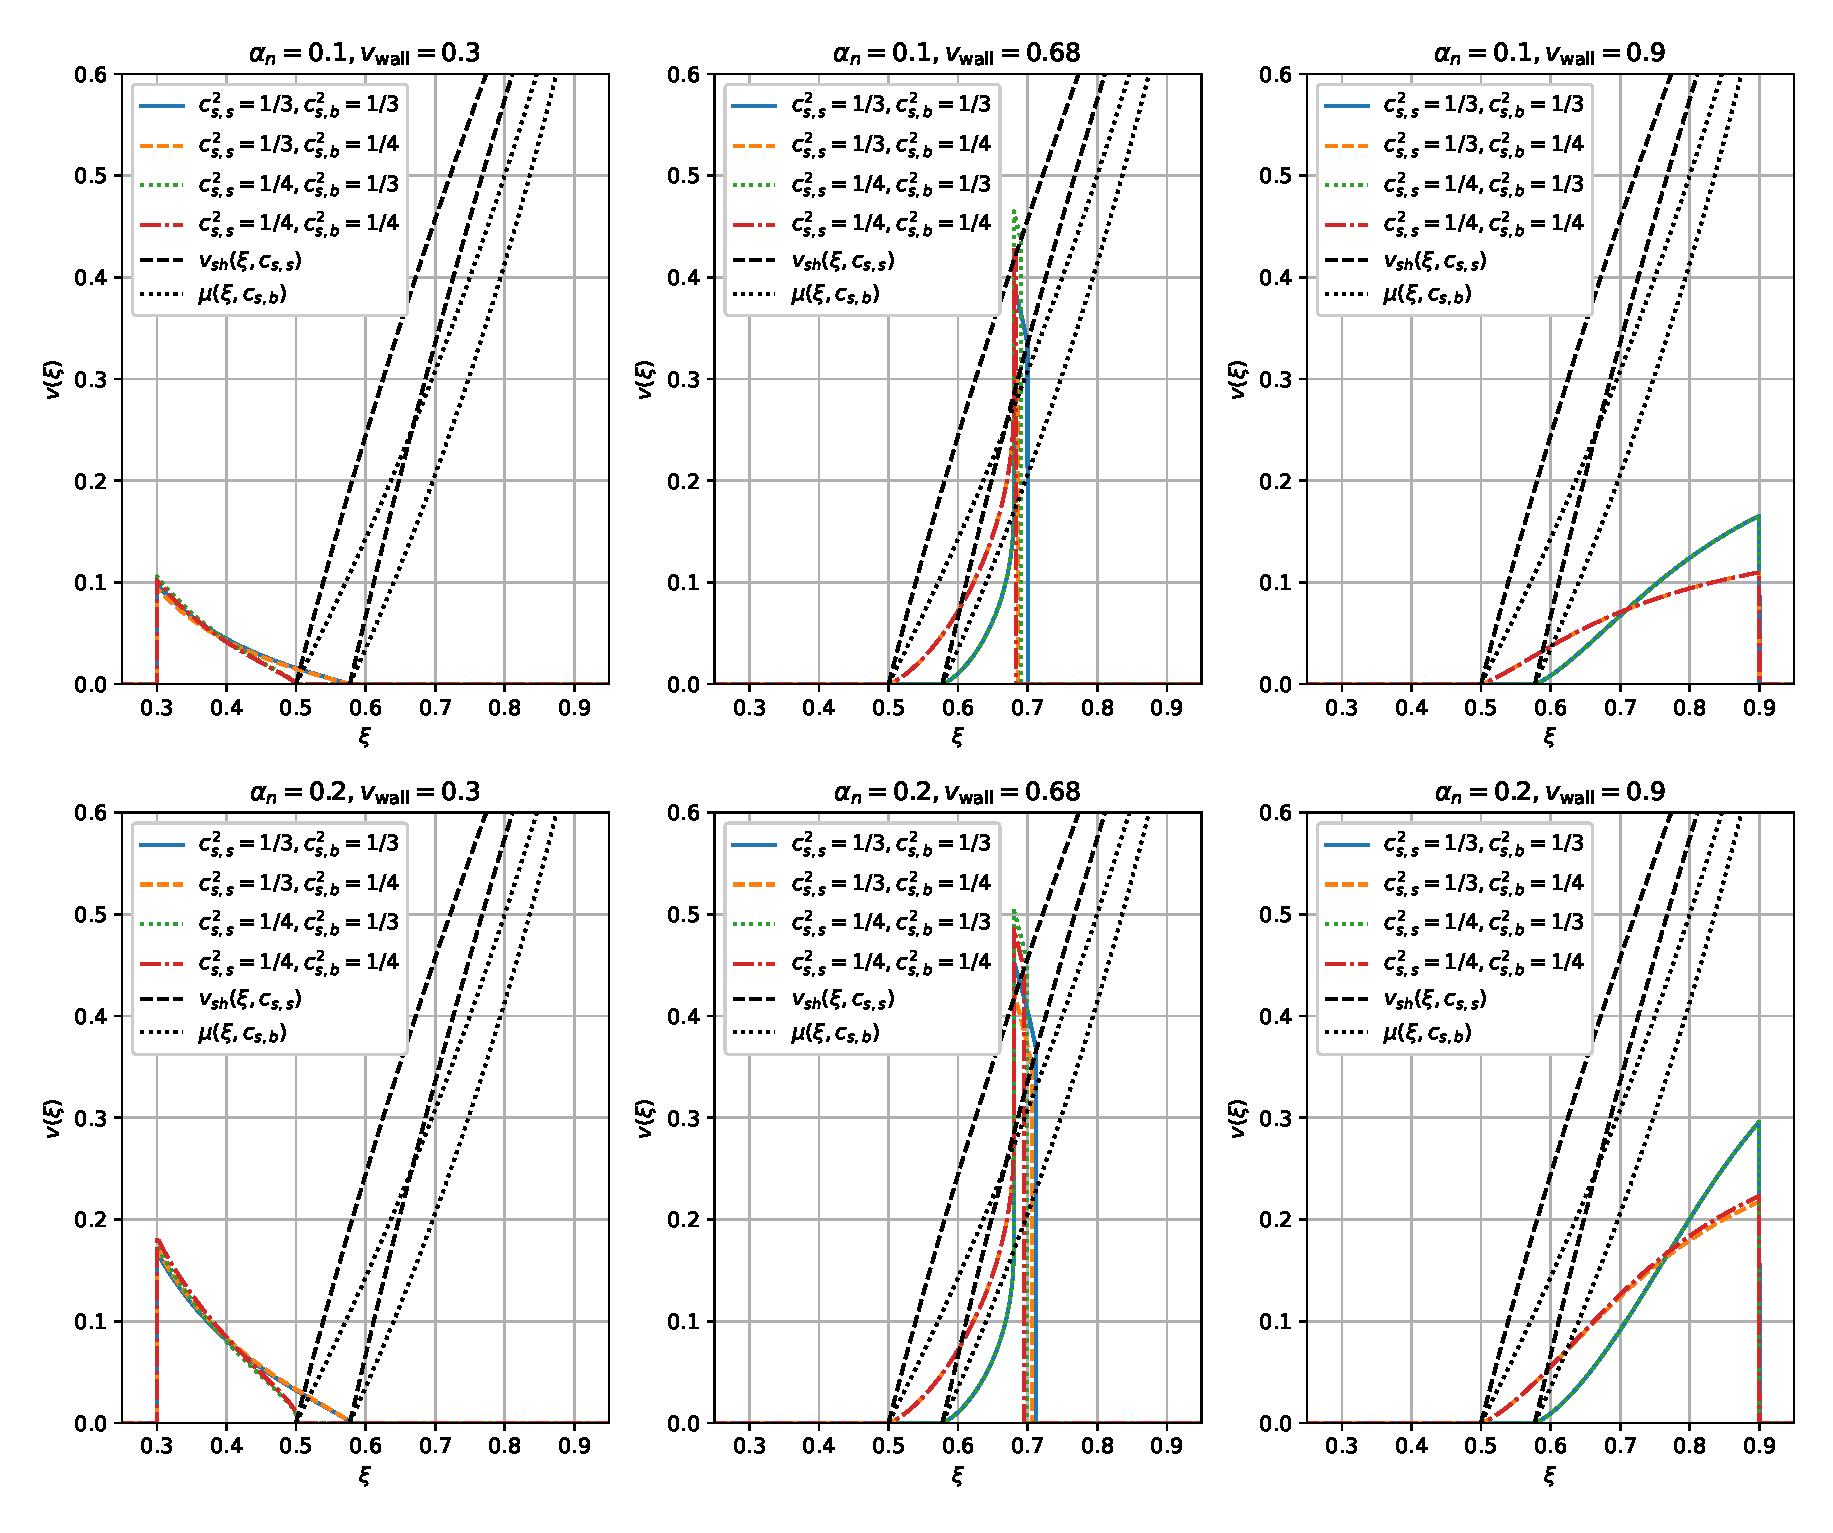
\includegraphics[width=\textwidth]{../pttools/examples/fig/const_cs_gw_v.eps}
\caption{Self-similar fluid profiles}
\label{fig:fluid_profiles}
\end{figure}

\begin{figure}[h!]
\centering
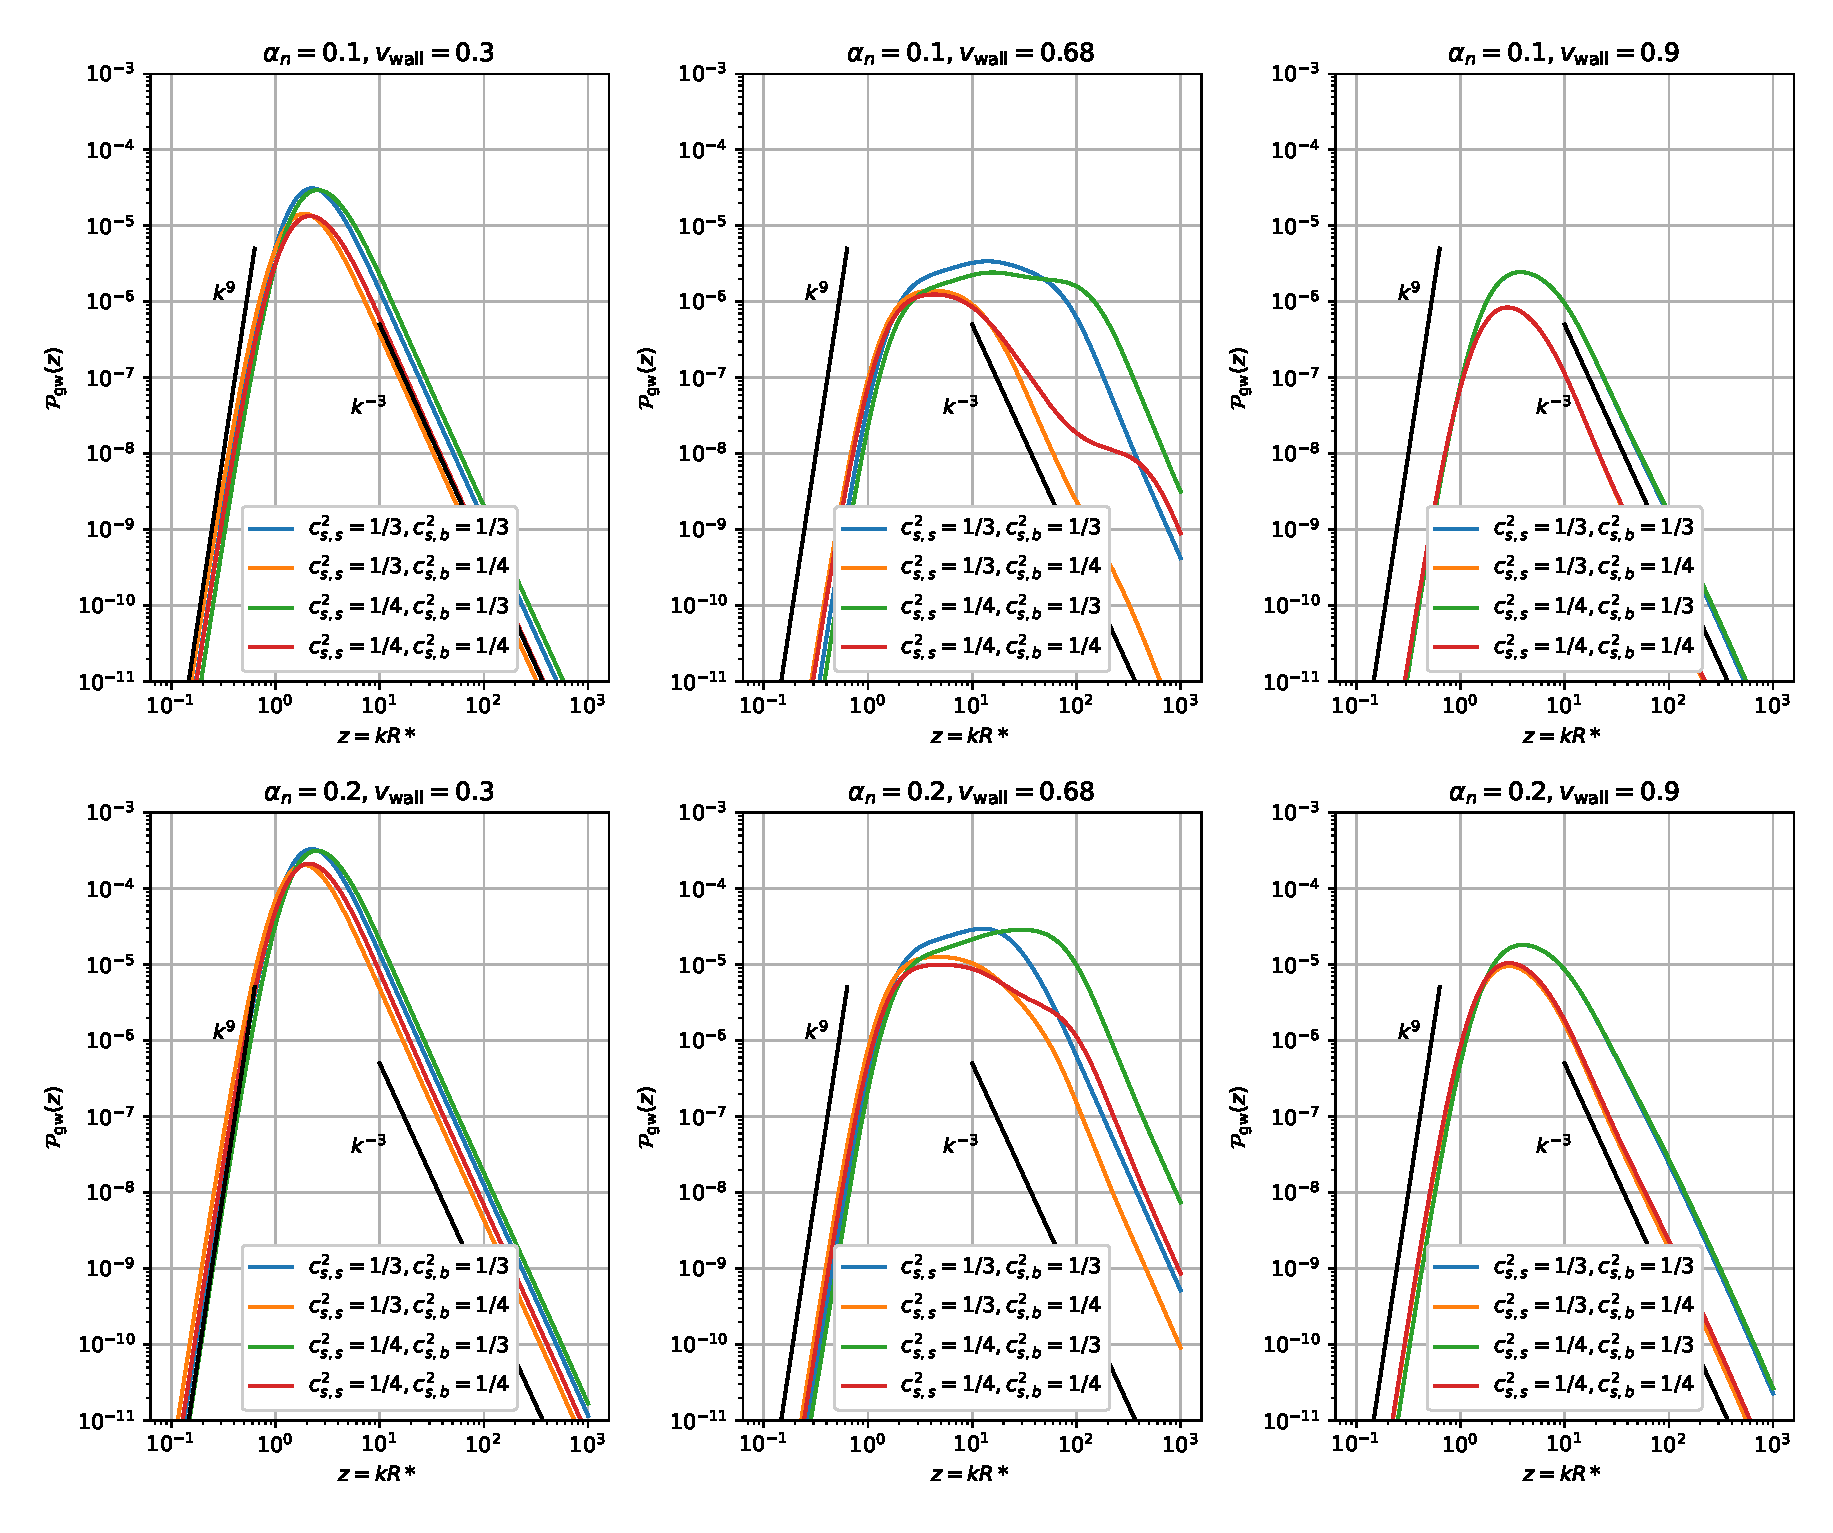
\includegraphics[width=\textwidth]{../pttools/examples/fig/const_cs_gw.eps}
\caption{Gravitational wave power spectra}
\label{fig:gw_spectra}
\end{figure}

\begin{figure}[h!]
\centering
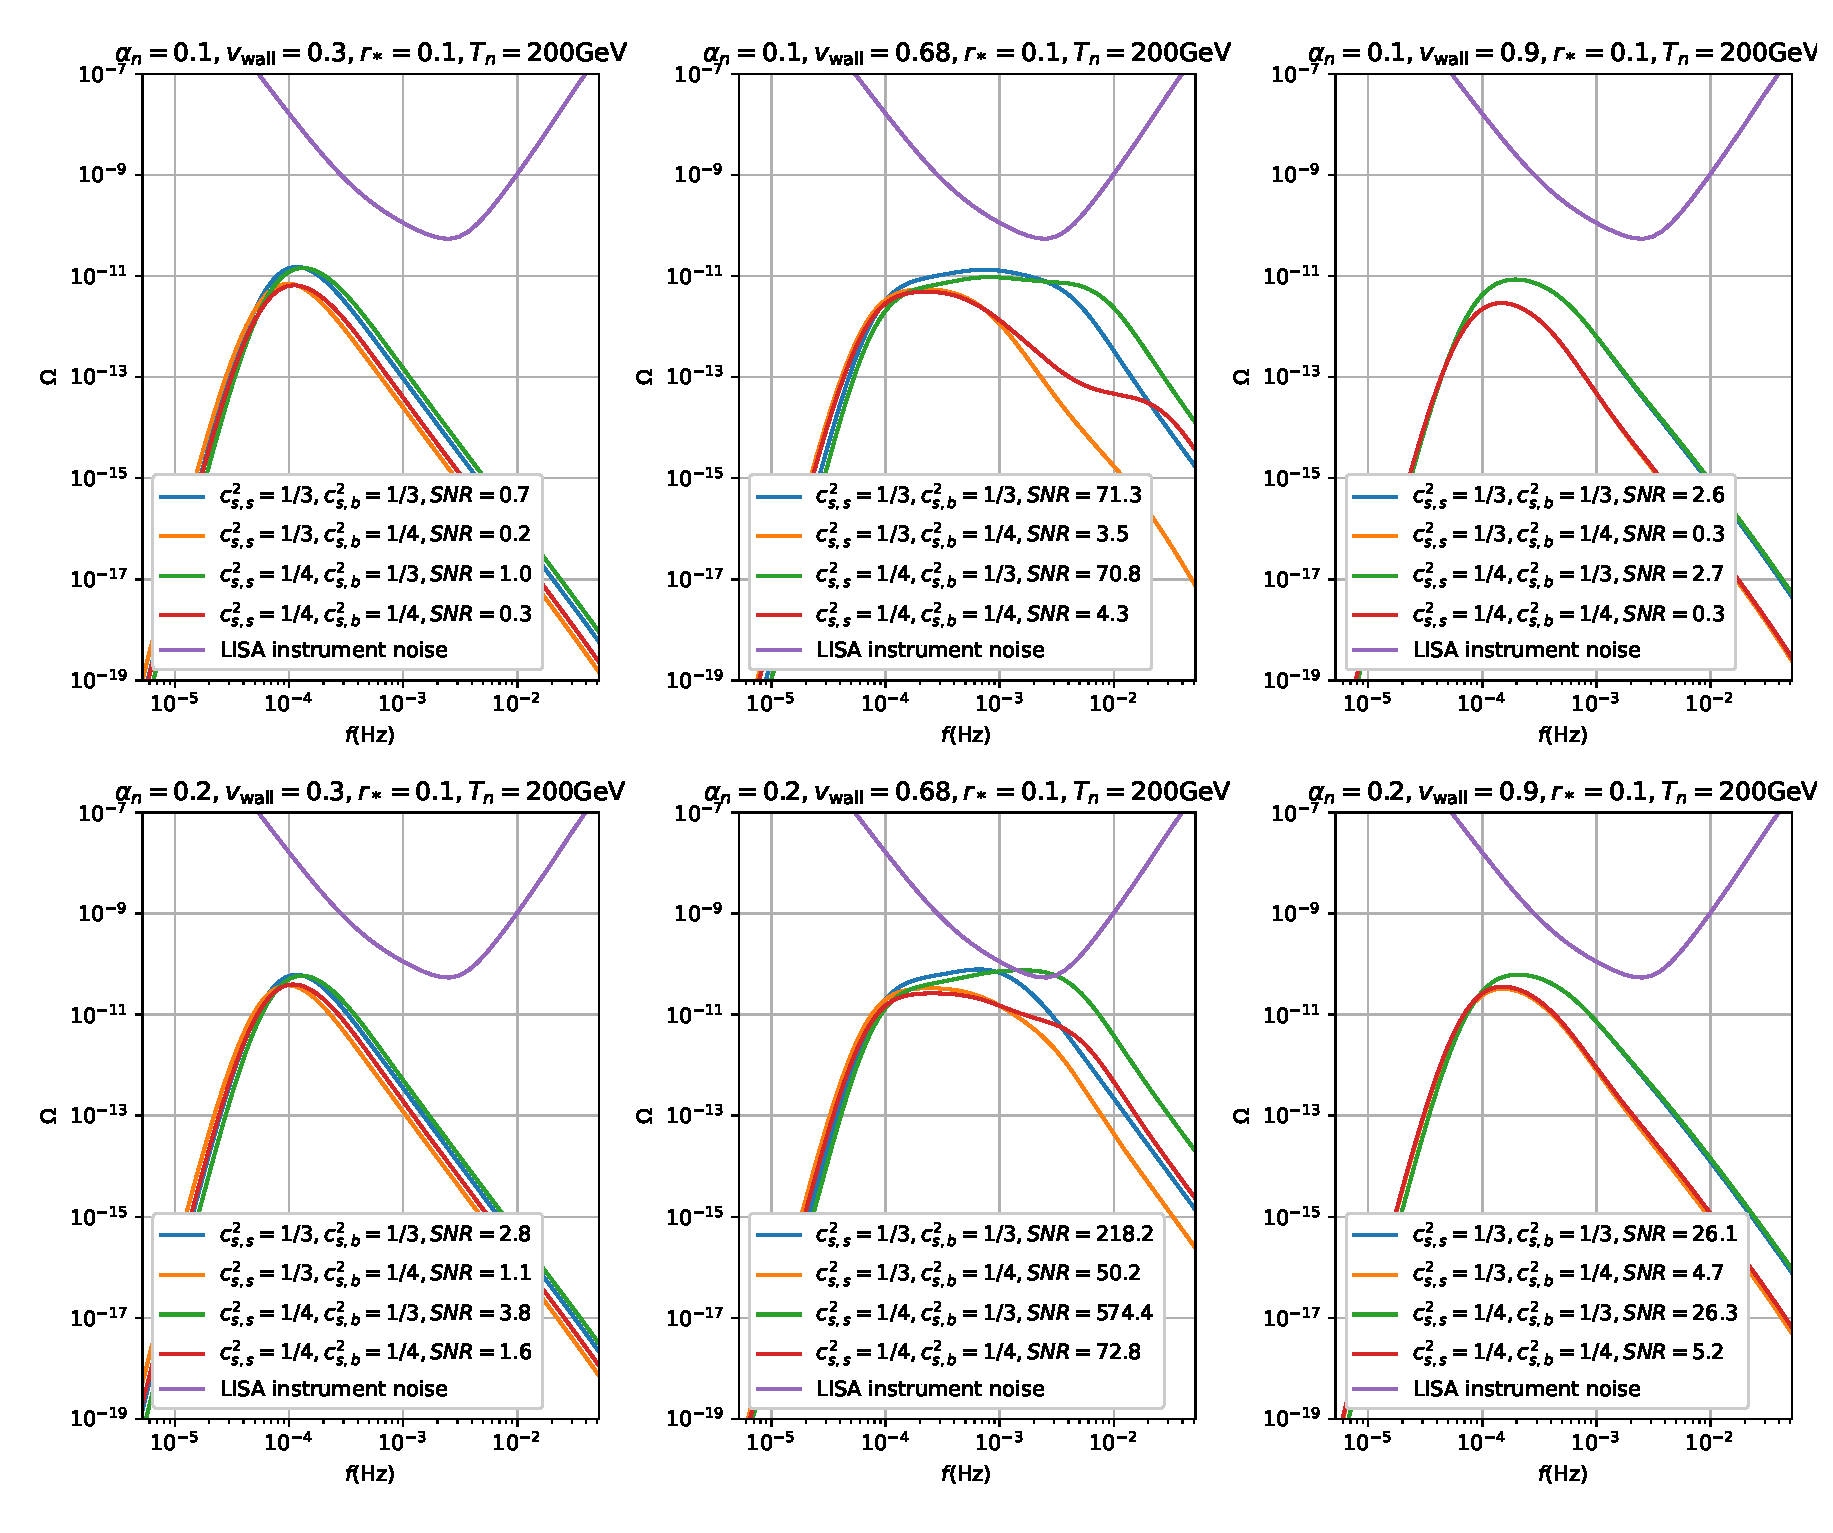
\includegraphics[width=\textwidth]{../pttools/examples/fig/const_cs_gw_omgw0.eps}
\caption{Gravitational wave power spectra today $\Omega_{gw,0}$}
\label{fig:omgw0}
\end{figure}

To test the precision and reliability of the results provided by PTtools,
we compared to the results in \cite[fig. 2]{giese_2021},
resulting in figure \ref{fig:kappa_giese}.
It should be noted that the article uses $\kappa_{\bar{\theta}_n}$ of eq. \eqref{eq:kappa_thetabar_n},
which differs from the $\kappa$ defined in eq. \eqref{eq:kappa_omega}.
The colors from blue to gray correspond to $\alpha = 0.01, 0.03, 0.1, 0.3, 1, 3$.
The figures on the left have $\alpha = \alpha_{\bar{\theta}_n}$
and the figures on the right have $\alpha = \alpha_n$.
For each color, the upper line has $c_{s,b}^2 = \frac{1}{3}$ and the lower line $c_{s,b}^2 = \frac{1}{4}$.
The solid lines correspond to $c_{s,s}^2 = \frac{1}{3}$ and the dashed lines correspond to $c_{s,s}^2 = \frac{1}{4}$.

\begin{figure}[h!]
\centering
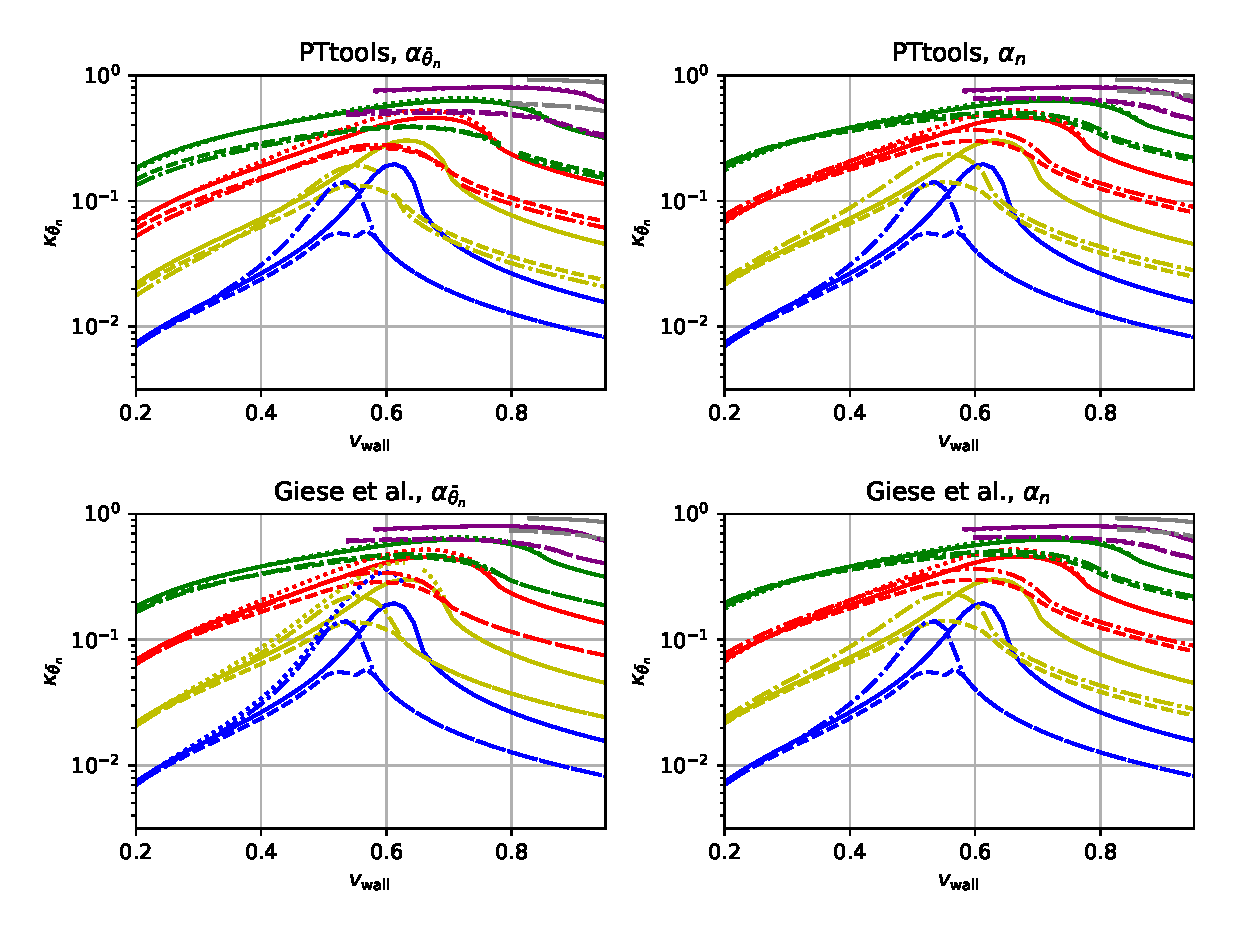
\includegraphics[width=\textwidth]{../pttools/examples/fig/giese_lisa_fig2.eps}
\caption{Comparison of $\kappa_{\bar{\theta}_n}$ values by \cite[fig. 2]{giese_2021} and PTtools}
\label{fig:kappa_giese}
\end{figure}
\todo{Use EPS instead of PNG}

It can be seen that PTtools and the code of \cite{giese_2021} produce results that are qualitativley similar, but slightly different.
This can be seen especially at the high wall speeds with $\alpha_n$ where changing $c_{s,s}$ (switching between the solid and dashed lines) has the opposite effect.

The gaps in the PTtools curves are caused by difficulties in finding a solution for very thin hybrid shells at the hybrid-detonation boundary.
It can happen that the shell is so thin that
It is also possible that the validity checks don't capture all the issues at this boundary,
resulting in a slightly wrong result.
This is demonstrated by the solid green $\alpha_n = 0.3, c_{s,s}^2 = \frac{1}{4}, c_{s,b} = \frac{1}{4}$ curve in the top-right figure.
These issues continue to be under investigation.

Some of the curves are not plotted by PTtools at all, since it has stricter tests for the validity of the bubble than the reference code.
One of such restrictions is that the $\alpha_n$ must be above the theoretical minimum for the model,
and that the model must have a valid critical temperature.
